\documentclass[letterpaper,12pt]{report}

\usepackage{graphicx}
\usepackage{hyperref}
\usepackage[top=1in, bottom=1in, left=1.25in, right=1in]{geometry}
\usepackage{float}
\usepackage{ltablex}
\usepackage[table]{xcolor}
\usepackage{array,ragged2e}

\setlength{\parindent}{0em}
\setlength{\parskip}{1em}

\renewcommand{\tabularxcolumn}[1]{m{#1}}
\newcolumntype{L}{>{\raggedright\arraybackslash}X}

\setcounter{tocdepth}{4}
\setcounter{secnumdepth}{4}
\renewcommand*\thesection{\arabic{section}}

\hypersetup{
    colorlinks, %set true if you want coloured links
    linkcolor=black,  %choose some colour if you want links to stand out
    citecolor=blue,
}

\begin{document}
    \begin{titlepage}
        \centering
        \vspace*{\fill}
        
\includegraphics[width=0.5\textwidth]{./diagrams/CarletonUniversityLogo.png}\par\vspace{2cm}
        {\scshape\Large SYSC3010 T3 Design Report\par}
        \vspace{1.5cm}
        {\huge\bfseries RC Camera Car\par}
        \vspace{2cm}
        {\large\itshape Alec D'Alessandro, 101033378\par}
        {\large\itshape Thao-Tran Le-Phuong, 100997443\par}
        {\large\itshape Honor Lopes, 101008909\par}
        {\large\itshape Igor Veselinovic, 101011081\par}
        \vspace*{\fill}

        {\large November 1, 2019\par}
    \end{titlepage}

    \begin{abstract}
        This document will restate the problem statement from the proposal. It
        will also outline the system design and software and hardware component
        designs for the project.
    \end{abstract}

    \tableofcontents

    \pagebreak

    \section{Problem Statement}

    The purpose of this project is to create a remote-controlled vehicle in
    order to explore locations that cannot be seen by the user. There are
    many locations inaccessible or unsafe for manned vehicles such as
    war zones, cave systems, and bio hazard spaces. These are locations where
    it would be unsafe to send human drivers and it would be preferable to
    send a remotely operated vehicle. This project would allow users to
    explore regions and places that are outside of their view.

    We would like to develop a basic version of the RC Camera Car for this
    project. The basic version should be a simple remote controlled car that
    connects over Wi-Fi and is easily controlled by a smart-phone app. This
    implementation could be expanded to work over a wireless communication
    technology so that the vehicle is less limited in range. Extended
    implementations would also include auxiliary equipment for performing
    specific tasks or covering a wider range of terrain. The basic version
    of this project would be suitable for recreational use. The extended
    version of this project could be applied in many fields such as science
    and military applications

    The overall goal for this project is for the car to be controlled via
    our designed Android application. Once the user has registered with the
    car through the application the main screen will be a live feed video
    source that is being transmitted from the car. The user will control the
    car using a Bluetooth connected game controller. The car could then be
    outfitted with additional auxiliaries needed for specific jobs. The car
    will also have automatic headlights to provide light in dimly lit areas.

    One limitation to the project development is how much bandwidth can be
    used for the live video feed stream from the car to the Android
    application. A proposed solution to this would be to decrease video
    resolution for bandwidth reducing purposes. A self-imposed constraint is
    on the complexity of the development of the car. This project will be
    focused on the vehicle controls and video feed. The car will be limited
    to Wi-Fi-enabled areas with even ground for this project. The Android
    app does not have to be connected to the same Wi-Fi as the car though,
    so the user can be in a different building and control the car.

    \section{System Design}

    \subsection{Deployment Diagram}

    The system design is shown in Figure \ref{fig:deployment}. The UML
    diagram outlines the components necessary for implementation and the
    relationships between them.

    Users will use the Android app to register their car to themselves and
    connect it to a Wi-Fi network. After the car is connected to Wi-Fi,
    users can control the car's movements via a game controller connected to
    the phone via Bluetooth as well as stream a video feed from and control
    the mounted camera. The video feed is to allow the user to control the
    car when it is not in sight. The app will also allow users to control
    the headlights of the car in case of dimly lit settings.

    There will be a Raspberry Pi that is connected to the Internet via
    Ethernet and acts as the centralized server. The server will have a
    database that will store the users, cars, and the pairings of users to
    cars. It will handle all of the commands coming from users and route
    them to their associated cars. Video feed from each car will be sent to
    the server to be streamed by the proper user.

    The body of the car will contain an Arduino and a Raspberry Pi. The
    Arduino will control the movement of the car (steering, acceleration) and
    handle the headlights of the car (photoresistor sensor and LEDs). The
    photoresistor sensors will be polled regularly to monitor the light
    intensity of an area and the Arduino will automatically turn the
    headlights (LEDs) on or off based on a threshold. The car movement will
    require motors to be connected to the Arduino and possibly a custom 3D
    printed chassis to hold all of the components. The car will use two rear
    wheels for propulsion along with a third wheel in the front that will
    balance the car. The Raspberry Pi will be connected to a Wi-Fi network to
    receive user commands and relay them to the Arduino via a wired
    connection. The Raspberry Pi will also be connected to the camera and
    will stream the video feed to the centralized server.

    \begin{figure}[H]
        \centering
        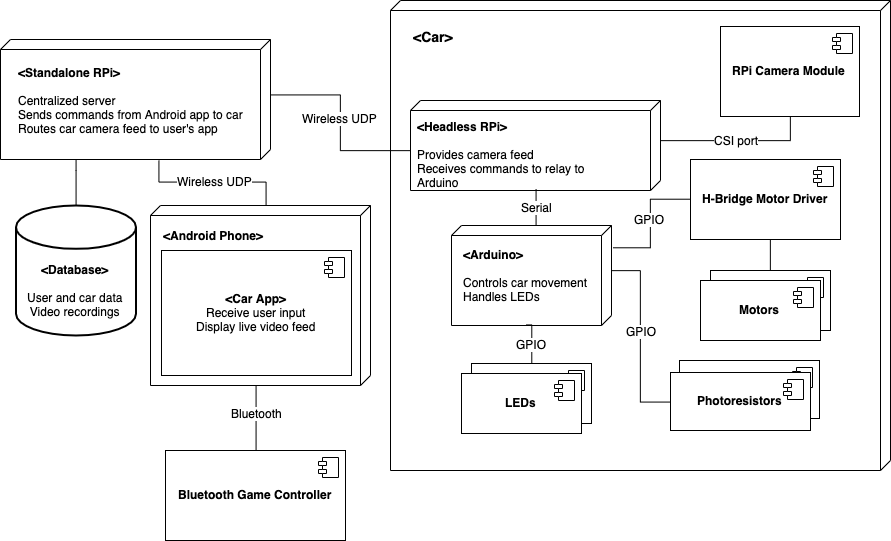
\includegraphics[width=0.9\linewidth]{diagrams/Design_Deployment_Diagram.png}
        \caption{Deployment diagram for RC car system}
        \label{fig:deployment}
    \end{figure}

    \subsection{Communication Protocols} \label{ssec:communication}

    The main use cases for the system are:
    \begin{itemize}
            \item User registration
            \item User login
            \item Car movement
            \item Video streaming
    \end{itemize}

    The communication protocols for the use cases are outlined below.

    \subsubsection{User Registration}

    During registration, the user will input into the Android app a name and
    password for their new account. The app will then pass the information to
    the server which will hash the password with a salt value and store the
    information in the database. The SQL library provides the ID of the last
    row modified, so the server will store the user ID locally as long as it
    is connected to the app. The user will then be prompted by the app to
    connect a car to a local Wi-Fi network. Once the car is connected, the
    car will respond to the app to confirm the connection with its name and
    IP address. The app will register the car with the system and send the
    car’s name and IP address to the server to be stored in the database
    along with the user’s ID. Once the server completes inputting the data
    into the database, it will respond to the app to confirm the
    registration.

    Figure \ref{fig:registration} is a sequence diagram of the process and Table
    \ref{table:registration} describes the communication protocols.

    \begin{figure}[H]
        \centering
        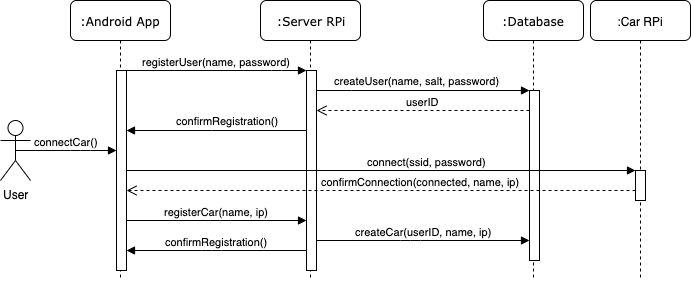
\includegraphics[width=0.9\linewidth]{diagrams/Design_Registration_Sequence.png}
        \caption{Sequence diagram of user registration}
        \label{fig:registration}
    \end{figure}

    \begin{tabularx}{\linewidth}
        {|>{\hsize=.5\hsize}L|>{\hsize=.5\hsize}L|>{\hsize=.8\hsize}L|L|}
    \caption{Communication protocols for user registration}
    \label{table:registration}\\
        \hline
        \centering\arraybackslash\textbf{Sender} &
        \centering\arraybackslash\textbf{Receiver} &
        \centering\arraybackslash\textbf{Message} &
        \centering\arraybackslash\textbf{Format}\\
        \hline
        Android App & Server RPi & register &
            \textbf{JSON object}\newline
            \{"name": string, "password": string, "carID": string\}\\
        \hline
        Server RPi & Database & createUser &
            \textbf{SQL query}\newline
            INSERT INTO users (name, salt, password) VALUES (?, ?, ?)\\
        \hline
        Database & Server RPi & userID &
            \textbf{int}\newline
            lastrowid attribute of sqlite cursor object\\
        \hline
        Server RPi & Android App & confirmRegistration &
            \textbf{JSON object}\newline
            \{"registered": boolean\}\\
        \hline
        Android App & Car RPi & connect &
            \textbf{JSON object}\newline
            \{"ssid": string, "password": string\}\\
        \hline
        Car RPi & Android App & confirmConnection &
            \textbf{JSON object}\newline
            \{"connected": boolean, "name": string, "ip": string\}\\
        \hline
        Android App & Server RPi & registerCar &
            \textbf{JSON object}\newline
            \{"name": string, "ip": string\}\\
        \hline
    \end{tabularx}

    \subsubsection{User Login}

    When a user logs in to the Android app, they will be prompted to provide
    their name and password that they used to register their account. The
    app will send this information to the server to be validated. The server
    will get the user information for the given name from the database and
    validate that the provided password matches the stored password. If it does
    not match, the server will inform the app that the inputted information
    was invalid. If it does match, the server will get all the car
    information that is associated with the user account and send the app a
    confirmation with the car information.

    There will be a limit to failed login attempts to protect against brute
    force hacking attacks. Once the limit is hit, the user will be locked out
    for a period of time that will increase with each successive lockout.

    Figure \ref{fig:login} is a sequence diagram of the login process and Table
    \ref{table:login} describes the communication protocols.

    \begin{figure}[H]
        \centering
        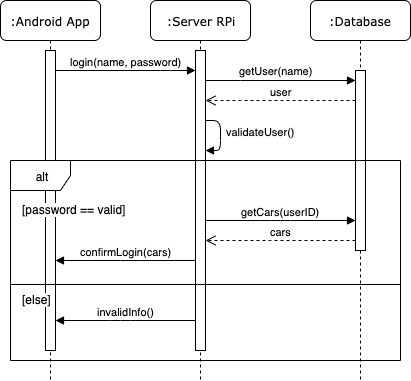
\includegraphics[width=0.7\linewidth]{diagrams/Design_Login_Sequence.png}
        \caption{Sequence diagram of user login}
        \label{fig:login}
    \end{figure}

    \subsubsection{Car Movement} \label{sssec:movement}

    To move the car, the user will move the joystick on the game controller
    that is connected to the Android phone via Bluetooth. When the Android
    app receives the movement event, it will send the joystick position to
    the server RPi which will then forward the message to the car RPi. The
    car RPi will then send the positioning to the car Arduino which will use
    that information to calculate the speed of the motors. The car Arduino
    will set the speeds of the left and right motors according to the results
    of the calculation.

    The server and car RPis will only pass the joystick position along if it
    is different from the previous position. This will protect against
    repeated packets so that the nodes are not overloaded by the increased
    number of packets.

    Figure \ref{fig:movement} is a sequence diagram of the movement process
    and Table \ref{table:movement} describes the communication protocols.

    \pagebreak

    \begin{tabularx}{\linewidth}
        {|>{\hsize=.5\hsize}L|>{\hsize=.5\hsize}L|>{\hsize=.8\hsize}L|L|}
    \caption{Communication protocols for user login}
    \label{table:login}\\
        \hline
        \centering\arraybackslash\textbf{Sender} &
        \centering\arraybackslash\textbf{Receiver} &
        \centering\arraybackslash\textbf{Message} &
        \centering\arraybackslash\textbf{Format}\\
        \hline
        Android App & Server RPi & login &
            \textbf{JSON object}\newline
            \{“name”: string, “password”: string\}\\
        \hline
        Server RPi & Database & getUser &
        \textbf{SQL query}\newline
        SELECT FROM users WHERE name=?\\
        \hline
        Database & Server RPi & user &
            \textbf{sqlite Row object}\newline
            \{id: int, name: string, salt: string, password: string\}\\
        \hline
        Server RPi & Database & getCar &
            \textbf{SQL query}\newline
            SELECT FROM cars WHERE userID=?\\
        \hline
        Database & Server RPi & cars &
            \textbf{sqlite Row objects}\newline
            \{id: int, userID: int, ip: string\}\\
        \hline
        Server RPi & Android App & confirmLogin &
            \textbf{JSON object}\newline
            \{“logged\_in”: boolean, cars: []\{“name”: string, “ip”: string\}\}\\
        \hline
        Server RPi & Android App & invalidInfo &
            \textbf{JSON object}\newline
            \{"error": string\}\\
        \hline
    \end{tabularx}

    \begin{figure}[H]
        \centering
        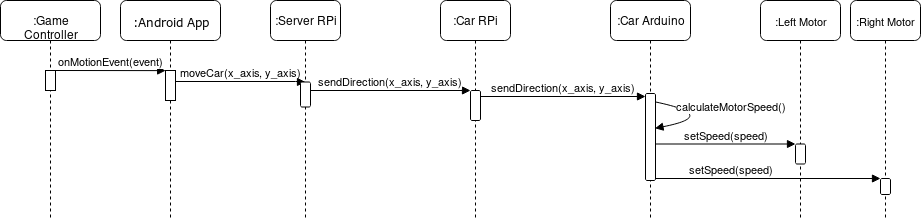
\includegraphics[width=\linewidth]{diagrams/Design_Car_Movement_Sequence.png}
        \caption{Sequence diagram of car movement control}
        \label{fig:movement}
    \end{figure}

    \pagebreak

    \begin{tabularx}{\linewidth}
        {|>{\hsize=.5\hsize}L|>{\hsize=.5\hsize}L|>{\hsize=.8\hsize}L|L|}
    \caption{Communication protocols for car movement}
    \label{table:movement}\\
        \hline
        \centering\arraybackslash\textbf{Sender} &
        \centering\arraybackslash\textbf{Receiver} &
        \centering\arraybackslash\textbf{Message} &
        \centering\arraybackslash\textbf{Format}\\
        \hline
        Game Controller & Android App & onMotionEvent &
            android.view.MotionEvent\newline
            (contains x and y axis values of controller joystick)\\
        \hline
        Android App & Server RPi & moveCar &
            \textbf{JSON object}\newline
            \{“x\_axis”: int, “y\_axis”: int\}\\
        \hline
        Server RPi / Car RPi & Car RPi / Car Arduino & sendDirection &
            \textbf{JSON object}\newline
            \{“x\_axis”: int, “y\_axis”: int\}\\
        \hline
        Car Arduino & Left Motor & setSpeed & [float from 0 to 255]\\
        \hline
        Car Arduino & Left Motor & setSpeed & [float from 0 to 255]\\
        \hline
    \end{tabularx}

    \subsubsection{Video Streaming} \label{sssec:stream}

    When the user selects a car to control, the Android app will access that
    car's video stream through an HTTP GET request. This request will be made
    to the server RPi which will route the request to the car RPi. The car
    RPi will respond with an HTML web page which the server RPi will then
    route back to the Android app. If the app is unable to access the video
    stream, it will display an error page to the user with suggestions on how
    to fix the issue.

    The sequence diagram of the process is shown in Figure \ref{fig:stream} and
    Table \ref{table:stream} describes the communication protocols.

    \begin{figure}[H]
        \centering
        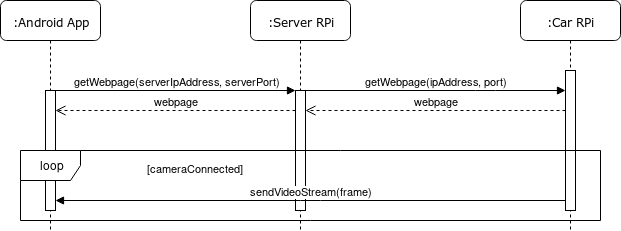
\includegraphics[width=0.75\linewidth]{diagrams/Design_Stream_Sequence.png}
        \caption{Sequence diagram of the video streaming process}
        \label{fig:stream}
    \end{figure}

    \begin{figure}[H]
        \begin{tabularx}{\linewidth}
            {|>{\hsize=.5\hsize}L|>{\hsize=.5\hsize}L|>{\hsize=.6\hsize}L|L|}
        \caption{Communication protocols for video streaming}
        \label{table:stream}\\
            \hline
            \centering\arraybackslash\textbf{Sender} &
            \centering\arraybackslash\textbf{Receiver} &
            \centering\arraybackslash\textbf{Message} &
            \centering\arraybackslash\textbf{Format}\\
            \hline
            Android App / Server RPi & Server RPi / Car Rpi & getWebpage &
                \textbf{HTTP Request}\newline
                GET https://\textless ipAddr\textgreater :\textless port\textgreater \\
            \hline
            Server RPi / Car RPi & Android App / Server RPi & webpage & HTML file\\
            \hline
            Car RPi & Android App & sendVideoStream & Video frame (bytes)\\
            \hline
        \end{tabularx}
    \end{figure}

    \subsubsection{General Error Handling}

    In the case of an error occurring during the communication between nodes,
    there will be a timeout when packets are sent so if a response is not
    received within this time, the request will be retried. This is to handle
    dropped packets. A node will also retry a packet if the response to a
    request is invalid.

    If the communication between nodes is broken, the app will display an error
    to the user with suggestions for fixing the issue, such as confirming
    internet connection of the Android phone or the car.

    \subsection{Database Schema}

    \begin{figure}[H]
        \centering
        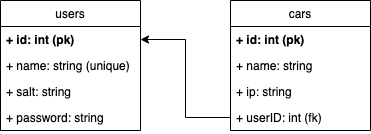
\includegraphics[width=0.7\linewidth]{diagrams/Design_Database_Schema.png}
        \caption{Database schema for storing users and their associated cars}
        \label{fig:database}
    \end{figure}

    The database schema for the system is shown in Figure \ref{fig:database}.
    There will be two tables: users, and cars.

    The “users” table will store the user information, which includes the
    user ID, name, salt, and password. The ID will be the primary key of the
    table. The stored password will be hashed and the salt will be used to
    validate login attempts. The name will be unique so each user must have a
    different name.

    Car information will be stored in the “cars” table. The car information
    would be the ID, name, IP address, and associated user ID. The ID will be
    the primary key of the table and the userID will be a foreign key to the
    “users” table.

    \section{Component Design}

    \subsection{Software}

    \subsubsection{Light-sensing \& Headlights}

    Figure \ref{fig:headlights} shows a flow chart describing the feedback loop
    of the light sensors and car headlights. The Arduino on the car polls the
    photoresistors on the car for its environment's brightness. If the
    environmental brightness is less than the defined brightness threshold
    constant, then the headlights are turned on. The headlights are turned off
    if the environmental brightness is greater than the threshold. This loop is
    repeated when the car is running. The LIGHTTHRESHOLD constant defines the
    brightness level where the car's headlights need to be turned on for the car
    to be operated safely.

    \subsubsection{Movement Control}

    The movement control of the car separates the concerns into two main
    categories: the user input and the actual rotation of the motors. The
    software running on the Arduino handles controlling the motors and expects
    to receive instructions in the form of JSON objects with an x and a y value,
    as defined in the Table \ref{table:movement} in section
    \ref{sssec:movement}. The source of instruction messages in this system is an
    Android application. The flow of a movement control message from the
    application to the motors can be seen in Figure \ref{fig:movement}, also in
    section \ref{sssec:movement}.

    The Android application takes input from a connected controller
    \cite{controller}. The application responds to input events from the
    controller and converts the input value(s) to x and y values that each
    range from a negative MIN value to a positive MAX value, with 0 being
    stationary. For example, if the input is from an analog joy-stick, then
    the set of possible input values for the joystick position is continuous,
    so the input values for x and y could get converted to any value between
    MIN and MAX. On the other hand, if the input is from a D-pad, then the
    set of possible input values is discrete (i.e, a directional input is
    either on or off at any given moment), so our Android application
    translates these on or off values to the appropriate value of MAX, MIN,
    or 0 for the x and y directions. The application then sends the converted
    x and y values in a JSON object. The Android application sends a new JSON
    instruction whenever the controller sends an input event from the analog
    joy-stick or D-pad.

    \begin{figure}[H]
        \centering
        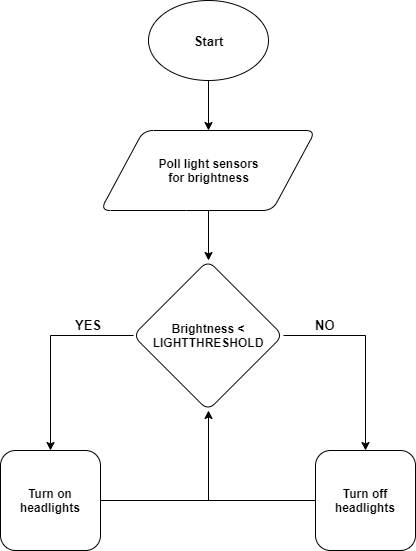
\includegraphics[width=0.6\linewidth]{diagrams/Headlights_Flowchart.png}
        \caption{Flow chart visualizing automatic headlight control algorithm}
        \label{fig:headlights}
    \end{figure}

    In order for the car to be able to go in a given direction with a given
    speed, the motors for each of the two wheels need to be spun either
    clockwise or counterclockwise at a certain rate. The JSON objects sent
    remotely to the car will have the aforementioned x and y values. The
    software running on the Arduino will use these two values to determine how
    to spin the motors in order to move in the corresponding direction.  For
    example, when receiving a JSON object with an x value of 0 and a y value of
    MAX, the software running on the Arduino will know to set both motors to
    spin at full forward speed. The Arduino will update the values being output
    to the motors whenever a new JSON instruction is received.

    \subsubsection{Video Streaming}

    The video stream recorded by the mounted Raspberry Pi camera will be
    served by an HTTP web server running on the car RPi. The web page served
    by the HTTP server will allow for any web browser on any machine on the
    same network as the car RPi to access the stream from the camera. The
    stream itself will be a Motion JPEG (mjpg) file that is embedded in the
    HTML web page. The web server will be based on the Web streaming example
    \cite{advancedrecipes} in the picamera Python package documentation. The
    Android application will use a WebView \cite{webbased} to display this
    web page in the app, so that user’s can see the video stream. Instead of
    requiring the Android app to access the video stream web page directly
    through the car RPi's IP address, a reverse proxy will be set up on the
    server RPi that will receive HTTP requests from the Android app and
    return the web page on behalf of the car's web server. This will simplify
    the implementation of the Android app because it only needs to know the
    server RPi's static IP address and doesn't need to worry about different
    IP addresses for different cars. The flow of messages between nodes is
    illustrated in Figure \ref{fig:stream} in section \ref{sssec:stream}.

    \subsubsection{Server Management}

    The server Raspberry Pi acts as a middle-man for this system. The server
    facilitates all communication between the Android application, the cars,
    and the database. Figure \ref{fig:vpn} below shows the network relationship between
    these components in the system and the presence of the VPN. This figure
    shows that the server, database, and multiple cars are within the VPN.

    Once deployed, the cars are expected to be connected to different
    networks than the device running the Android application. This VPN allows
    for a connection between the application and the distributed cars,
    through the middle-man server. This VPN is required in order to avoid
    having the cars be publicly available over the internet. Having the
    cars publicly accessible could create a security risk with the video
    livestream available to watchers who have accessed the port. The VPN can
    be seen in figure 8 above as the grey cloud element surrounding the cars,
    server, and database. The device running the Android application is not
    within the VPN cloud.

    The server Raspberry Pi acts as a middle-man between the system
    components. This involves facilitating routines between the cars and
    applications, and the application and database. These routines have been
    described in section \ref{ssec:communication} above including the User
    Registration protocol, the Car Registration protocol and the User Login
    protocol. The server is used as an intermediate in sending movement
    control and video streaming between the cars and the android application.
    In these software protocols, all information sent is passed through the
    server.


    \begin{figure}[H]
        \centering
        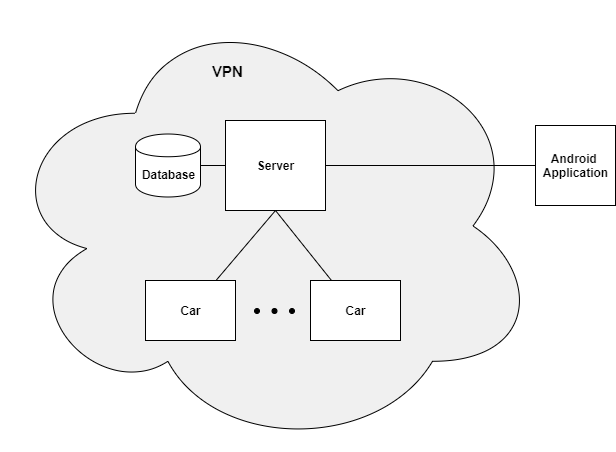
\includegraphics[width=\linewidth]{diagrams/VPN.png}
        \caption{Diagram showing the VPN used in the system}
        \label{fig:vpn}
    \end{figure}

    \subsection{Hardware}

    \subsubsection{Schematics}

    The overall design of the remote car is shown in Figure \ref{fig:hardware}
    with the components laid out from a birds eye view. Starting in the top
    left of the image with the breadboard, there are two yellow LEDs followed by
    resistors, which are connected to digital outputs from the Arduino.
    Additionally there are three photoresistors each associated with their own
    resistor. These photoresistors are connected to the analog inputs on the
    Arduino. Two motors are used for controlling the direction of the vehicle.
    They are shown in the middle slightly to the right and are connected to a
    motor driver. The Arduino is in series with the motor driver, that will send
    digital signals to the motor driver. The driver will then decode these
    signals to state the direction of rotation for the motors. On the right side
    of the figure is the power cell used for the car, which will be four AAA
    batteries. Please note the software used to create diagram only had four AA
    battery holder.

    \textbf{Legend for Wires coming from the Arduino:}
    \begin{itemize}
        \item Blue, Green, Pink, Yellow - Signals being sent to Driver Motor
        \item Cyan - Connection for Photoresistor 2
        \item Dark Brown, Dark Purple - Supplementary power being sent to Driver Motor
        \item Grey - Connection for LED 1
        \item Light Brown - Connection for Photoresistor 3
        \item Orange - Connection for LED 2 and Photoresistor 1
    \end{itemize}

    \textbf{Legend for Wires coming from the Driver Motor:}
    \begin{itemize}
        \item Green - Positive side of Motor 1
        \item Grey - Positive side of Motor 2
        \item Red - Negative side of Motors 1 and 2
    \end{itemize}

    \textbf{Legend for Battery Bank:}
    \begin{itemize}
        \item Black - Positive terminal of battery
        \item Red to Yellow - Negative terminal of battery
    \end{itemize}

    \begin{figure}[H]
        \centering
        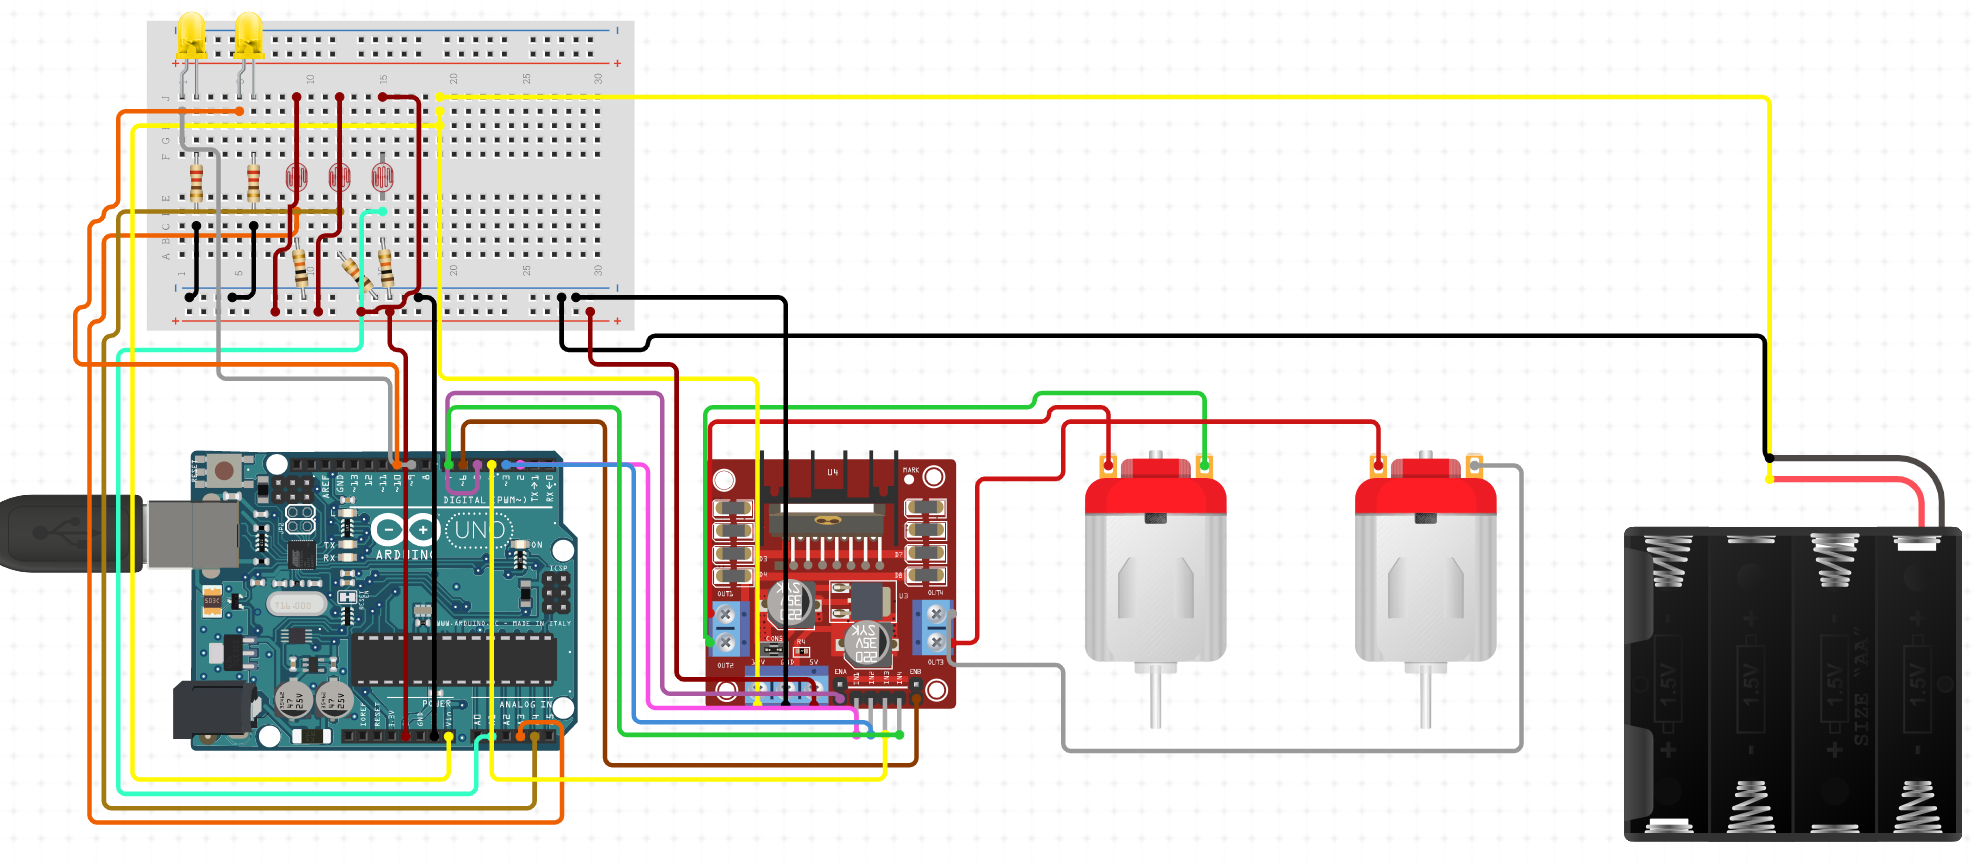
\includegraphics[width=\linewidth]{diagrams/Design_Hardware_Schematic.png}
        \caption{Overview of hardware and wiring of remote car}
        \label{fig:hardware}
    \end{figure}

    \subsection{Testing Protocol}

    Each time the car is powered on it goes through a test protocol to ensure
    all the components are in working order. This procedure runs a simple script
    in the following order of hardware components created by the developers.

    \subsubsection{Headlights}

    This will ensure that each headlight is being powered correctly. This is a
    simplified view of the test being implemented for the left and right
    headlight of the car. The test is performed on each LED individually.

    \textbf{Procedure:}
    \begin{enumerate}
        \item Repeat the following three times:
            \begin{enumerate}
                \item Turn LED on
                \item Turn LED off
            \end{enumerate}
    \end{enumerate}

    \subsubsection{Motors}

    During the testing sequence of the motor it will ensure that rotation for
    each motor are in full working order. The test has 2 parts for it to be
    completed correctly. Part one ensures the motor is capable of completing a
    full rotation clockwise, while part two is completing a full rotation
    counter-clockwise. The test is done on each motor individually so the user
    can visually see if the motors are in working order.

    \textbf{Procedure:}
    \begin{enumerate}
        \item Rotate motor clockwise a full rotation
        \item Rotate motor counter-clockwise a full rotation
    \end{enumerate}

    \subsubsection{Camera}

    This test is completed after the phone has established a connection with the
    car, so that the user will have access to see if the video streaming from
    the car is in working order.

    \begin{figure}
        \textbf{Procedure:}
        \begin{enumerate}
            \item Power camera on
            \item Initiate a recording
            \item Wait 3 seconds
            \item Stop the recording
            \item Turn off camera
        \end{enumerate}
    \end{figure}

    \subsubsection{Photoresistors}

    The test will check three photoresistors and provide feedback that it's
    reading correctly. In our design, we are including three photoresistors on
    various places on the car to get an average across the car, to verify that
    the entire car is in a dark location to turn the headlight on and not a
    photoresistor in a shadow.

    \textbf{Procedure:}
    \begin{enumerate}
        \item  Give power to the photoresistor
        \item Read the value of the photoresistor
        \item Ensure that the value is neither 0 nor 1023
    \end{enumerate}

    The test validates that the value from the photoresistor is not zero nor
    1023 to ensure it’s in working order. As the photoresistor should never
    produce a value of zero even in the darkest of locations. With the
    resistance value that was chosen, using ambient light it should not produce
    a value of 1023 which is also the maximum value.

    \begin{thebibliography}{9}
        \bibitem{controller}
        “Handle controller actions,” Android developers. [Online]. Available:
        \\\url{https://developer.android.com/training/game-controllers/controller-input}

        \bibitem{advancedrecipes}
        D. Jones, “4. Advanced Recipes,” Picamera. [Online]. Available:
        \\\url{https://picamera.readthedocs.io/en/latest/recipes2.html#web-streaming}

        \bibitem{webbased}
        “Web-based content,” Android developers. [Online]. Available:
        \\\url{https://developer.android.com/guide/webapps}
    \end{thebibliography}

\end{document}
